%\VignetteEngine{knitr::knitr}
%\VignetteIndexEntry{Flexible Logo plots of symbols and alphanumeric strings using Logolas}
%\VignettePackage{Logolas}

% To compile this document
% library('knitr'); rm(list=ls()); knit('Logolas/vignettes/logolas.Rnw')
% library('knitr'); rm(list=ls()); knit2pdf('Logolas/vignettes/logolas.Rnw'); openPDF('logolas.pdf')
% !Rnw weave = knitr

\documentclass[12pt]{article}

\newcommand{\Logolas}{\textit{Logolas}}
\usepackage{dsfont}
\usepackage{cite}



\RequirePackage{/Library/Frameworks/R.framework/Versions/3.3/Resources/library/BiocStyle/resources/tex/Bioconductor}

\AtBeginDocument{\bibliographystyle{/Library/Frameworks/R.framework/Versions/3.3/Resources/library/BiocStyle/resources/tex/unsrturl}}



\author{Kushal K Dey \\[1em]
\small{\textit{Stephens Lab}, Dept. of Statistics, The University of Chicago} \mbox{ }\\
\small{\texttt{$^*$Correspondending Email: kkdey@uchicago.edu}}}


\bioctitle[ Flexible Logo plots of symbols and alphanumeric strings using \Logolas{}]{Flexible Logo plots of symbols and alphanumeric strings using \Logolas{}}

\begin{document}

\maketitle

\begin{abstract}
\vspace{1em}
Logo plots are popular in genomic studies for sequence alignment and motif detection. However, logo plots have been restrictive in its scope due to limited size of the library of symbols used by logo plotting tools and packages  and the lack of flexibility in extending it to other applications. In this package, we provide an easy and flexible interface for the user to plot logos. More importantly, we extend the library of logos from A, C, T, G (library of symbols in seqLogo) and English alphabets (library of symbols in RWebLogo, motifStack) to include numbers and alpha-numeric strings with provision for punctuations and arrows. It also provides the user with a simple graphical interface to create her own logo and add to her personal library.
In this vignette, we discuss a number of applications in genomics and beyond where such flexible logo plots can be effective in visualizing patterns.

\vspace{1em}
\textbf{\Logolas{} version:} 0.99.2 \footnote{This document used the vignette from \Bioconductor{} package \Biocpkg{CountClust, DESeq2} as \CRANpkg{knitr} template}
\end{abstract}



\newpage

\tableofcontents

\section{Introduction}

Logo plots are a popular tool in bioinformatics and regulatory genomics studies for representing sequence alignment patterns and for sequence and protein motif detection. One of the first and widely used logo plotting tools is \Biocpkg{seqLogo} by Oliver Bembom \cite{Bembom2016}, specifically targeted at DNA sequence alignment. However, it has a library of only 4 symbols - A, C, G and T- corresponding to the 4 nucleotides. The package \CRANpkg{RWebLogo} is an extension of WebLogo python package that plots custom sequence logos by extending it to all alphabets \cite{Wagih2014}. Another package \Biocpkg{motifStack} works with both DNA/RNA sequence motif and amino acid sequence motif and customizes font size and colors \cite{Ou2015}.

\Logolas{} adds more flexibility by customizing logos and the graphical design of the logo plots. Also it extends the library of symbols beyond English alphabets to numbers, symbols (arrows, punctuations) and to alphanumeric strings. It allows the user to choose a range of information criteria to determine logo sizes. It provides a simple user interface to create new logos and add them to their personalized library of logos and even apply them in strings. We show several applications in genomics, ecology and document mining, where such logo plots can be applied.

\newpage

\section{\Logolas{} Installation}

\Logolas{} requires the following CRAN-R package : \CRANpkg{grid}, \CRANpkg{gridExtra}, \CRANpkg{RColorBrewer}, \CRANpkg{devtools}.

\begin{knitrout}
\definecolor{shadecolor}{rgb}{0.969, 0.969, 0.969}\color{fgcolor}\begin{kframe}
\begin{alltt}
\hlkwd{source}\hlstd{(}\hlstr{"http://bioconductor.org/biocLite.R"}\hlstd{)}
\hlkwd{biocLite}\hlstd{(}\hlstr{"Logolas"}\hlstd{)}
\end{alltt}
\end{kframe}
\end{knitrout}

For the developmental version on Github, one can use

\begin{knitrout}
\definecolor{shadecolor}{rgb}{0.969, 0.969, 0.969}\color{fgcolor}\begin{kframe}
\begin{alltt}
\hlstd{devtools}\hlopt{::}\hlkwd{install_github}\hlstd{(}\hlstr{'kkdey/Logolas'}\hlstd{)}
\end{alltt}
\begin{verbatim}
## '/Library/Frameworks/R.framework/Resources/bin/R' CMD INSTALL '/private/var/folders/0f/v6kp3_hj7rd2wrhms9mf4h500000gn/T/RtmpVdKbyo/devtools138528b79e04/kkdey-Logolas-00e489f'
\end{verbatim}
\end{kframe}
\end{knitrout}

Then load the package with:

\begin{knitrout}
\definecolor{shadecolor}{rgb}{0.969, 0.969, 0.969}\color{fgcolor}\begin{kframe}
\begin{alltt}
\hlkwd{library}\hlstd{(Logolas)}
\end{alltt}
\end{kframe}
\end{knitrout}

\section{Applications}

We start with the most basic application of logo plots - for alignment of DNA sequence, comprising of logos A, C, T and G, corresponding to the four nucleotide. This is the typical application of \Biocpkg{seqLogo}. We start with the same demo example provided in the \Biocpkg{seqLogo} vignette.

\begin{figure}[h]
\begin{center}
\begin{knitrout}
\definecolor{shadecolor}{rgb}{0.969, 0.969, 0.969}\color{fgcolor}\begin{kframe}
\begin{alltt}
\hlstd{mFile} \hlkwb{<-} \hlkwd{system.file}\hlstd{(}\hlstr{"Exfiles/pwm1"}\hlstd{,} \hlkwc{package}\hlstd{=}\hlstr{"seqLogo"}\hlstd{)}
\hlstd{m} \hlkwb{<-} \hlkwd{read.table}\hlstd{(mFile)}
\hlstd{p} \hlkwb{<-} \hlstd{seqLogo}\hlopt{::}\hlkwd{makePWM}\hlstd{(m)}
\hlstd{seqLogo}\hlopt{::}\hlkwd{seqLogo}\hlstd{(p)}
\end{alltt}
\end{kframe}
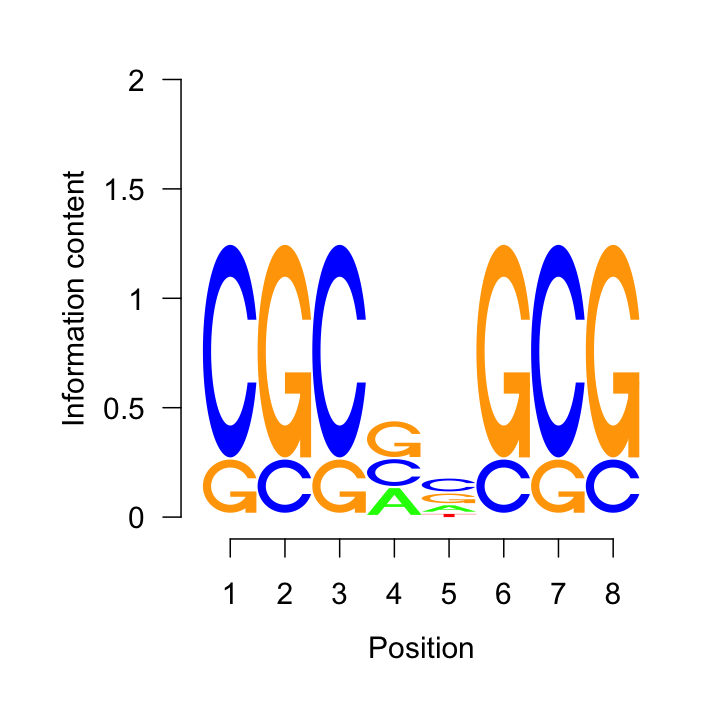
\includegraphics[width=5in,height=5in]{figure/seqlogo_use-1} 

\end{knitrout}
\end{center}
\end{figure}


The user first needs to make a position weight matrix from the matrix using the \begin{verb} makePWM() \end{verb} function. Then it uses the \begin{verb} seqLogo() \end{verb} function on the output to plot the logo plots.

\newpage

Now we apply \Logolas{} to build similar plot. We start with the same matrix as in \Biocpkg{seqLogo}, and assign row names and column names that will be used in the plot as symbols and block labels respectively.

\begin{figure}[h]
\begin{center}




































